\documentclass[a4paper, 12pt]{article}

%%% Работа с русским языком
\usepackage{cmap}					% поиск в PDF
\usepackage{mathtext} 				% русские буквы в формулах
\usepackage[T2A]{fontenc}			% кодировка
\usepackage[utf8]{inputenc}			% кодировка исходного текста
\usepackage[russian]{babel}	% локализация и переносы

%%% Дополнительная работа с математикой
\usepackage{amsmath,amsfonts,amssymb,amsthm,mathtools} % AMS
\usepackage{icomma} % "Умная" запятая: $0,2$ --- число, $0, 2$ --- перечисление

%% Номера формул
%\mathtoolsset{showonlyrefs=true} % Показывать номера только у тех формул, на которые есть \eqref{} в тексте.

%% Шрифты
\usepackage{euscript}	 % Шрифт Евклид
\usepackage{mathrsfs} % Красивый матшрифт

%% Поля
\usepackage[left=2cm,right=2cm,top=2cm,bottom=2cm,bindingoffset=0cm]{geometry}

%% Русские списки
\usepackage{enumitem}
\makeatletter
\AddEnumerateCounter{\asbuk}{\russian@alph}{щ}
\makeatother

%%% Работа с картинками
\usepackage{graphicx}  % Для вставки рисунков
\graphicspath{{images/}{images2/}}  % папки с картинками
\setlength\fboxsep{3pt} % Отступ рамки \fbox{} от рисунка
\setlength\fboxrule{1pt} % Толщина линий рамки \fbox{}
\usepackage{wrapfig} % Обтекание рисунков и таблиц текстом

%%% Работа с таблицами
\usepackage{array,tabularx,tabulary,booktabs} % Дополнительная работа с таблицами
\usepackage{longtable}  % Длинные таблицы
\usepackage{multirow} % Слияние строк в таблице

%% Красная строка
\setlength{\parindent}{2em}

%% Интервалы
\linespread{1}
\usepackage{multirow}

%% TikZ
\usepackage{tikz}
\usetikzlibrary{graphs,graphs.standard}

%% Верхний колонтитул
\usepackage{fancyhdr}
\pagestyle{fancy}

%% Перенос знаков в формулах (по Львовскому)
\newcommand*{\hm}[1]{#1\nobreak\discretionary{}
	{\hbox{$\mathsurround=0pt #1$}}{}}

%% Мои дополнения
\usepackage{float} %Добавляет возможность работы с командой [H] которая улучшает расположение на странице
\usepackage{gensymb} %Красивые градусы
\usepackage{graphicx}               % Импорт изображений
\usepackage{caption} % Пакет для подписей к рисункам, в частности, для работы caption*


\begin{document}

\newcommand{\HRule}{\rule{\linewidth}{0.7mm}} % Defines a new command for the horizontal lines, change thickness here
	
	\begin{center}
		\large\textbf{Московский Физико-Технический Институт}\\
		\large\textbf{(государственный университет)}
	
		\vfill
		
		\Large Лабораторная работа по курсу общей физики № 3.2.8\\[0.5cm] % Minor heading such as course title
		
		%----------------------------------------------------------------------------------------
		%	TITLE SECTION
		%----------------------------------------------------------------------------------------
		
		\HRule
		\\[0.4cm]
		{ \huge \bfseries Релаксационные колебания}
		\\[0.4cm] % Title of your document
		\HRule
		\\[0.5cm]
		
		\ \\
	\textbf{\large Автор:} \\	
	\large Баранников Андрей Б01-001\\
		\vfill
		\hspace*{-0.8 cm}
\includegraphics[width=100 pt]{frkt_logo}\\
		\large Долгопрудный, 2021
	\end{center}

\newpage
\setcounter{page}{2}
\fancyfoot[c]{\thepage}
\fancyhead[L] {Работа 3.2.8}
\fancyhead[R]{}

	\paragraph*{Цель работы:} изучение петель гистерезиса ферромагнитных материалов с помощью осциллографа.

\paragraph*{Оборудование:} автотрансформатор, понижающий трансформатор, амперметр и вольтметр (мультиметры), резистор, делитель напряжения, интегрирующая
цепочка, электронный осциллогра, тороидальные образцы с двумя обмотками..

\section{Теоретическое введение}

\begin{wrapfigure}{l}{0.6\textwidth}
	\vspace{-20pt}
	\begin{center}
		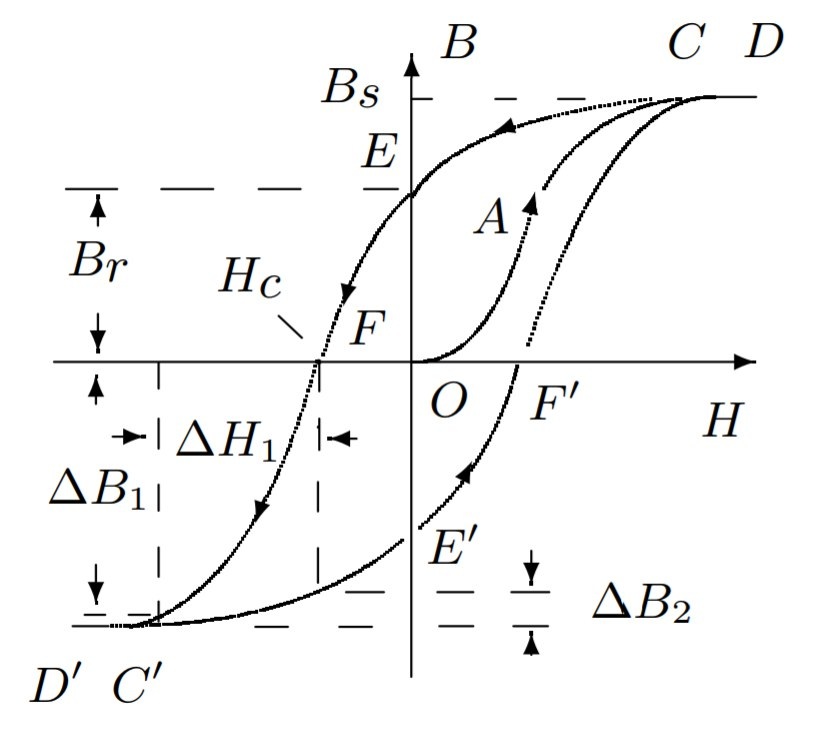
\includegraphics[width=0.7\linewidth]{Image_1.jpeg}
		\label{fig:sdfsafd}
	\end{center}
	\vspace{-10pt}
	\caption{Петля гистерезиса ферромагнетика}
\end{wrapfigure}

Магнитная индукция $\vec{B}$ и напряженность магнитного поля
$\vec{H}$ в ферромагнитном материале неоднозначно связаны
между собой: индукция зависит не только от напряженности, но
и от предыстории образца. Связь между индукцией
и напряженностью поля типичного ферромагнетика иллюстрирует рис. 1. Если
к размагниченному образцу начинают прикладывать магнитное поле, то его намагничивание следует кривой $ OACD $, выходящей
из начала
координат. Эту кривую называют \textit{основной кривой намагничивания}.


Индукция $\vec{B}$ в образце состоит из индукции, связанной с намагничивающим полем
$\vec{B}$, и индукции, создаваемой самим намагниченным
образцом.
В системе СИ эта связь имеет вид

$$\vec{B} = \mu_{0}(\vec{H}+\vec{M}),$$

где $\vec{M}$- \textit{намагниченность} - магнитный момент единичного объема образца, а $\mu_{0}$ - магнитная постоянная.

Намагнитим образец до насыщения - до точки D. Соответствующее
значение индукции $B_{s}$ называют индукцией насыщения. При уменьшении поля $H$ до нуля зависимость $B(H)$ имеет вид кривой $DCE$, и при нулевом поле индукция имеет конечное ненулевое значение. Это остаточная индукция $B_{r}$ . Чтобы размагнитить образец, то есть перевести его в состояние
$F$, необходимо приложить "обратное" магнитное
поле $H_{c}$, которое называют коэрцитивной силой.

Замкнутая кривая $DEFD'E'F'D$, возникающая при циклическом
перемагничивании образца, намагниченного до насыщения, называется \textit{предельной петлей гистерезиса.}


\subsection{Измерение магнитной индукции в образцах.}
Магнитную индукцию удобно определять с помощью ЭДС, возникающей при изменении магнитного потока Ф в катушке, намотанной на образец:

$$\mathscr{E} = -\dfrac{dФ}{dt}.$$

Тогда отсюда и из формулы $Ф=BSN_{и}$ получаем:
$$|B|=\dfrac{1}{SN_{и}}\int \mathscr{E}dt.$$
Для интегрирования сигнала применяют интегрирующие схемы (рис. 2).

\begin{wrapfigure}{l}{0.6\textwidth}
	\vspace{-20pt}
	\begin{center}
		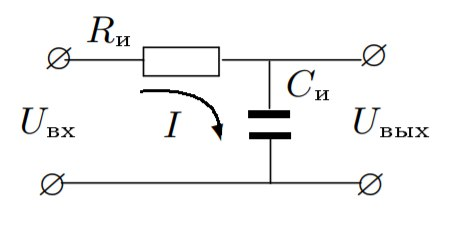
\includegraphics[width=0.7\linewidth]{Image_2.jpeg}
		\label{fig:sdfsafd}
	\end{center}
	\vspace{-10pt}
	\caption{Интегрирующая RC-цепь}
\end{wrapfigure}

Если выходной сигнал намного меньше входного ($U_{вых}\ll U_{вх},$) ток в цепи пропорционален входному напряжению: $I\simeq\dfrac{U_{вх}}{R}$, а напряжение на емкости С

$$U_{вых}\simeq\dfrac{1}{RС}\int U_{вх}dt.$$

Этот вывод тем ближе к истине, чем больше постоянная $\tau=RC$ превосходит характерное время процесса (например, его период). Для синусоидальных напряжений

$$U_{вых}=\dfrac{U_{вх}}{RC\Omega},$$

где $\Omega$ - частота сигнала.

В итоге, обозначив параметры интегрирующей цепи через $R_{и}$ и $C_{и}$, получаем

$$ |B|=\dfrac{1}{SN_{и}}\int U_{вх}dt=\dfrac{R_{и}С_{и}}{SN_{и}}U_{вых}.$$

\section{Экспериментальная установка.}
Схема экспериментальной установки показана на рис. 3.

Действующее значение переменного тока в обмотке N0 измеряется амперметром А (мультиметром GDM). Последовательно с амперметром включено сопротивление $R_{0}$, напряжение с которого подается на вход X электронного осциллографа (ЭО). Это напряжение пропорционально току в обмотке $N_{0}$, а следовательно и напряженности H магнитного поля в образце.

Для измерения магнитной индукции B с измерительной обмотки $N_{И}$ на вход интегрирующей RC -цепочки подается напряжение $U_{И}$ (UВХ), пропорциональное производной $\dot{B}$, а с выхода снимается напряжение $U_{C}$($U_{ВЫХ}$), пропорциональное
величине B , и подается на вход Y осциллограа.
Замкнутая кривая, возникающая на экране, воспроизводит в некотором масштабе (различном для осей X и Y ) петлю гистерезиса. Чтобы придать этой кривой количественный смысл, необходимо установить масштабы изображения, т.е. провести калибровку каналов X и Y ЭО. Для этого, во-первых, надо узнать, каким напряжениям (или токам) соответствуют амплитуды сигналов, видимых на экране, и во-вторых,  каким значениям B и H соответствуют эти напряжения
(или токи).

\begin{figure}[H]
	\centering
	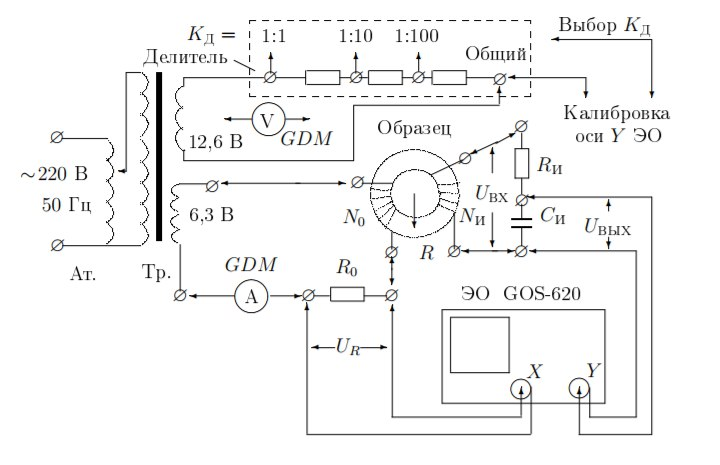
\includegraphics[width=\linewidth]{Image_3.jpeg}
	\caption{Схема установки для исследования намагничивания образцов}
	\label{fig:Holl2}
\end{figure}

\section{Ход работы}

\begin{enumerate}
	\item Запишем данные установки:
	
	$R_{0}=0,2 \, Ом \ \ R_{и}=20 \, кОм \ \ С_{и}=20 \, мкФ $
	
	Параметры тороидальных образцов:
	
	\begin{itemize}
		
		\item	\textbf{Пермаллой ($ Fe-Ni $  НП50)}: $N_{0}=15$ витков;
		$N_{и}=300$ витков;
		$S=0,66 \, см^{2}$;
		$2\pi R = \, 14,1 см $.  
		
		\item	\textbf{Феррит 1000нн}: $N_{0}=45$ витков;
		$N_{и}=400$ витков;
		$S=3,0 \, см^{2}$;
		$2\pi R = 25 \, см $.  
	\end{itemize}
	
	
	\item Соберем схему (рис. 3) и настроим оборудование. 	
	
	\item Для каждого образца сфотографируем предельную петлю. Запишем значения коэффициентов усиления $K_{x}$ и $K_{y}$, ток $I_{эф}$. Измерим двойные амплитуды для коэрцитивной силы $2x(c)$ и индукции насыщения $2y(s)$. Результаты таковы:
	
	\begin{itemize}
		
		\item 	\textbf{Пермаллой}:
		
		$K_{x}=10 \dfrac{мВ}{дел},$
		$K_{y}=10 \dfrac{мВ}{дел},$
		$I_{эф}=226 мА. $
		При этом $ 2x = 7 дел, \; 2y = 3,5 дел$.
		
		\item 	 \textbf{Феррит}:
		
		$K_{x}=20 \dfrac{мВ}{дел},$
		$K_{y}=20 \dfrac{мВ}{дел},$
		$I_{эф}=92,6 мА. $
		При этом $ 2x = 2,1 дел, \; 2y = 8 дел$.
		
		\newpage
		
		
	\end{itemize}
	
	
	
	\item Снимем для каждого образца начальную кривую намагничивания (табл. 1-3), плавно уменьшая ток до нуля и отмечая вершины частных петель. По этим данным построим эти кривые (рис. 4-6).
	
	\begin{table}[h!]
		\caption{Начальная кривая намагничивания для феррита}
		\begin{center}
			\begin{tabular}{|c|c|c|c|c|c|c|} 
				\hline 
				№ &  1 &  2 & 3 & 4 & 5 &  6   \\ 	\hline
				
				$ x $, дел & 2.0 & 1.9 & 1.8 & 1.7 & 1.6 & 0.95  \\
				$ y $, дел & 8 & 7 & 6 & 5 & 3.6 & 2  \\
				\hline
				
			\end{tabular}
		\end{center}
	\end{table}
	

	
	
	\begin{table}[h!]
		\caption{Начальная кривая намагничивания для пермаллоя}
		\begin{center}
			\begin{tabular}{|c|c|c|c|c|c|c|} 
				\hline 
				№ &  1 &  2 & 3 & 4 & 5 &  6    \\ 	\hline
				
				$ x $, дел & 3.6 & 3.2 & 2.8 & 2.4 & 2.2 & 1.8  \\
				$ y $, дел & 6 & 6 & 4.2 & 2.2 & 1 & 0.2  \\
				\hline
				
			\end{tabular}
		\end{center}
	\end{table}

\begin{figure}[h!]
	\centering
	\includegraphics[scale=0.5]{Image_4}
	\caption{Петля гистерезиса для феррита}
\end{figure}

\newpage

\begin{figure}[h!]
	\centering
	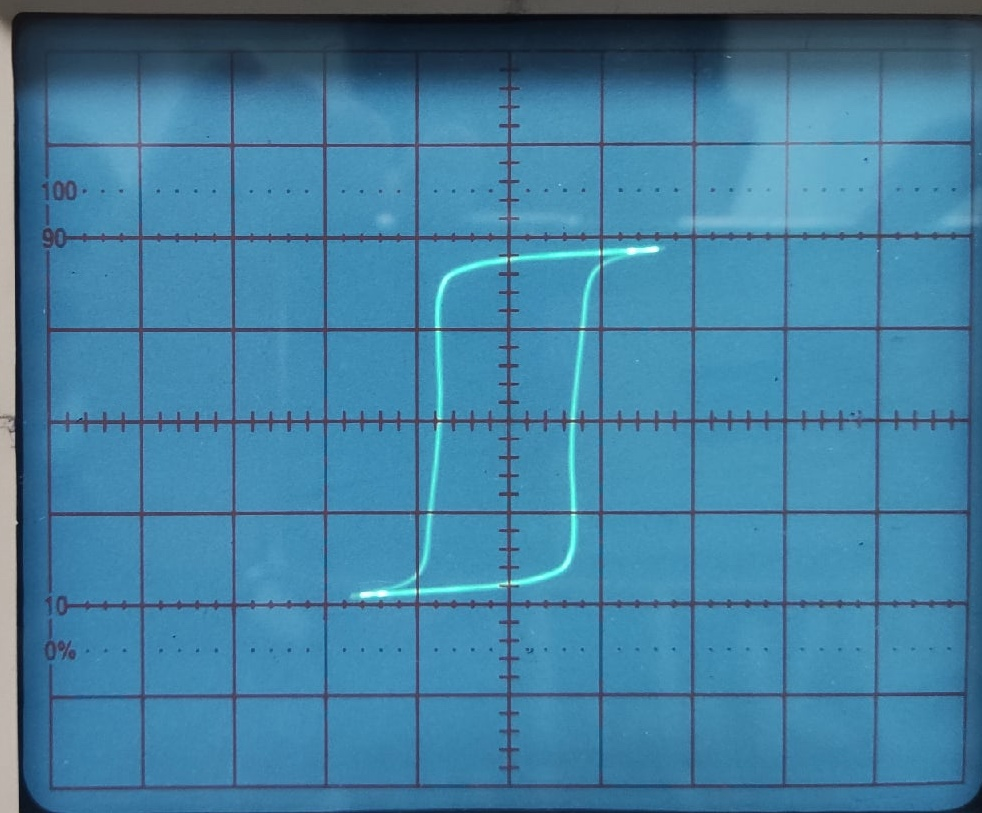
\includegraphics[scale=0.3]{Image_5.jpeg}
	\caption{Петля гистерезиса для пермаллоя}
\end{figure}

\item  Рассчитаем  цену деления ЭО для петли для оси Х (в $\dfrac{А}{м}$) по формуле:

$$H=\dfrac{IN_{0}}{2\pi R},$$

где $I=\dfrac{K_{x}}{R_{0}}$, и в Теслах на деление для оси Y по формуле

$$B=\dfrac{R_{и}С_{и}U_{вых}}{SN_{и}},$$

где $U_{вых}=K_{y}.$


\begin{itemize}
	
	\item	\textbf{Пермаллой}:
	
	$H=10,64 \dfrac{А}{м}.$
	$B=0,4 \dfrac{Т}{дел}.$
	
	\item	\textbf{Феррит}:
	
	$H=9,0 \dfrac{А}{м}.$
	$B=3,33 \cdot 10^{-2} \dfrac{Т}{дел}.$
	
\end{itemize}

\section{Обработка результатов}

\item Рассчитаем значения $m_x$ и $m_y$  и сравним с величинами $K_x$ и $K_y$, использованными при калибровке: \\
\[
m_x = \frac{2 R_0 \sqrt{2}I_{ЭФ} }{2x} \frac{В}{дел}
\]
\[
m_y = \frac{2 \sqrt{2}U_{ЭФ} }{2y} \frac{В}{дел}
\]

\[
I_{ЭФ} = 0,4 \, A; \; 2x = 8,4 \, дел \Rightarrow m_x = 0,027 \, \frac{В}{дел}, \; K_x = 20 \, мВ 
\]
\[
U_{ЭФ} = 0,111 \, В; \; 2y = 13 \, дел \Rightarrow m_y = 0,024 \, \frac{В}{дел}, \; K_y = 20 \, мВ 
\]

Значения $m_x$ и $m_y$ совпадают с величинами $K_x$ и $K_y$ в пределах погрешности. \\

\item Сравним постоянную времени $\tau = RC$, с расчётом через параметры  $R_и$  и $C_и$: \\
\[
\tau = RC = U_{ВХ} / (\Omega U_{ВЫХ}) 
\]
\[
U_{ВХ} = 5,2 \, В; \; U_{ВЫХ} = 0,287 \, В; \; \tau \approx 0,36; \; R_И C_И = 0,4
\]
Значения $\tau$ и $R_И C_И$ совпадают в пределах погрешности.
\[
R = 20 \cdot 10^3 \, Ом \gg \frac{1}{\Omega C} = 159 \, c
\]
С достаточной точностью выполняется условие $R \gg 1/(\Omega C)$
\item Рассчитаем коэрцитивную силу $H_c$ и индукцию насыщения $B_S$ для каждого образца:\\

\begin{itemize}
	
	\item	\textbf{Пермаллой}:
	
	\fbox{$H_{c}=19,2 \pm 0,5 \dfrac{А}{м}$}
	\fbox{$B_{s}=1,20 \pm 0,06 \ Тл$}
	
	\item	\textbf{Феррит}:
	
	\fbox{$H_{c}=9,0 \pm 0,2 \dfrac{А}{м}$}
	\fbox{$B_{s}=(13,30\pm 0,02) \cdot 10^{-2} Тл$}
\end{itemize}


\item Оценим максимальные значения дифференциальной магнитной проницаемости $\mu_{max}$ по начальным кривым намагничивания:

\begin{figure}[h!]
	\centering
	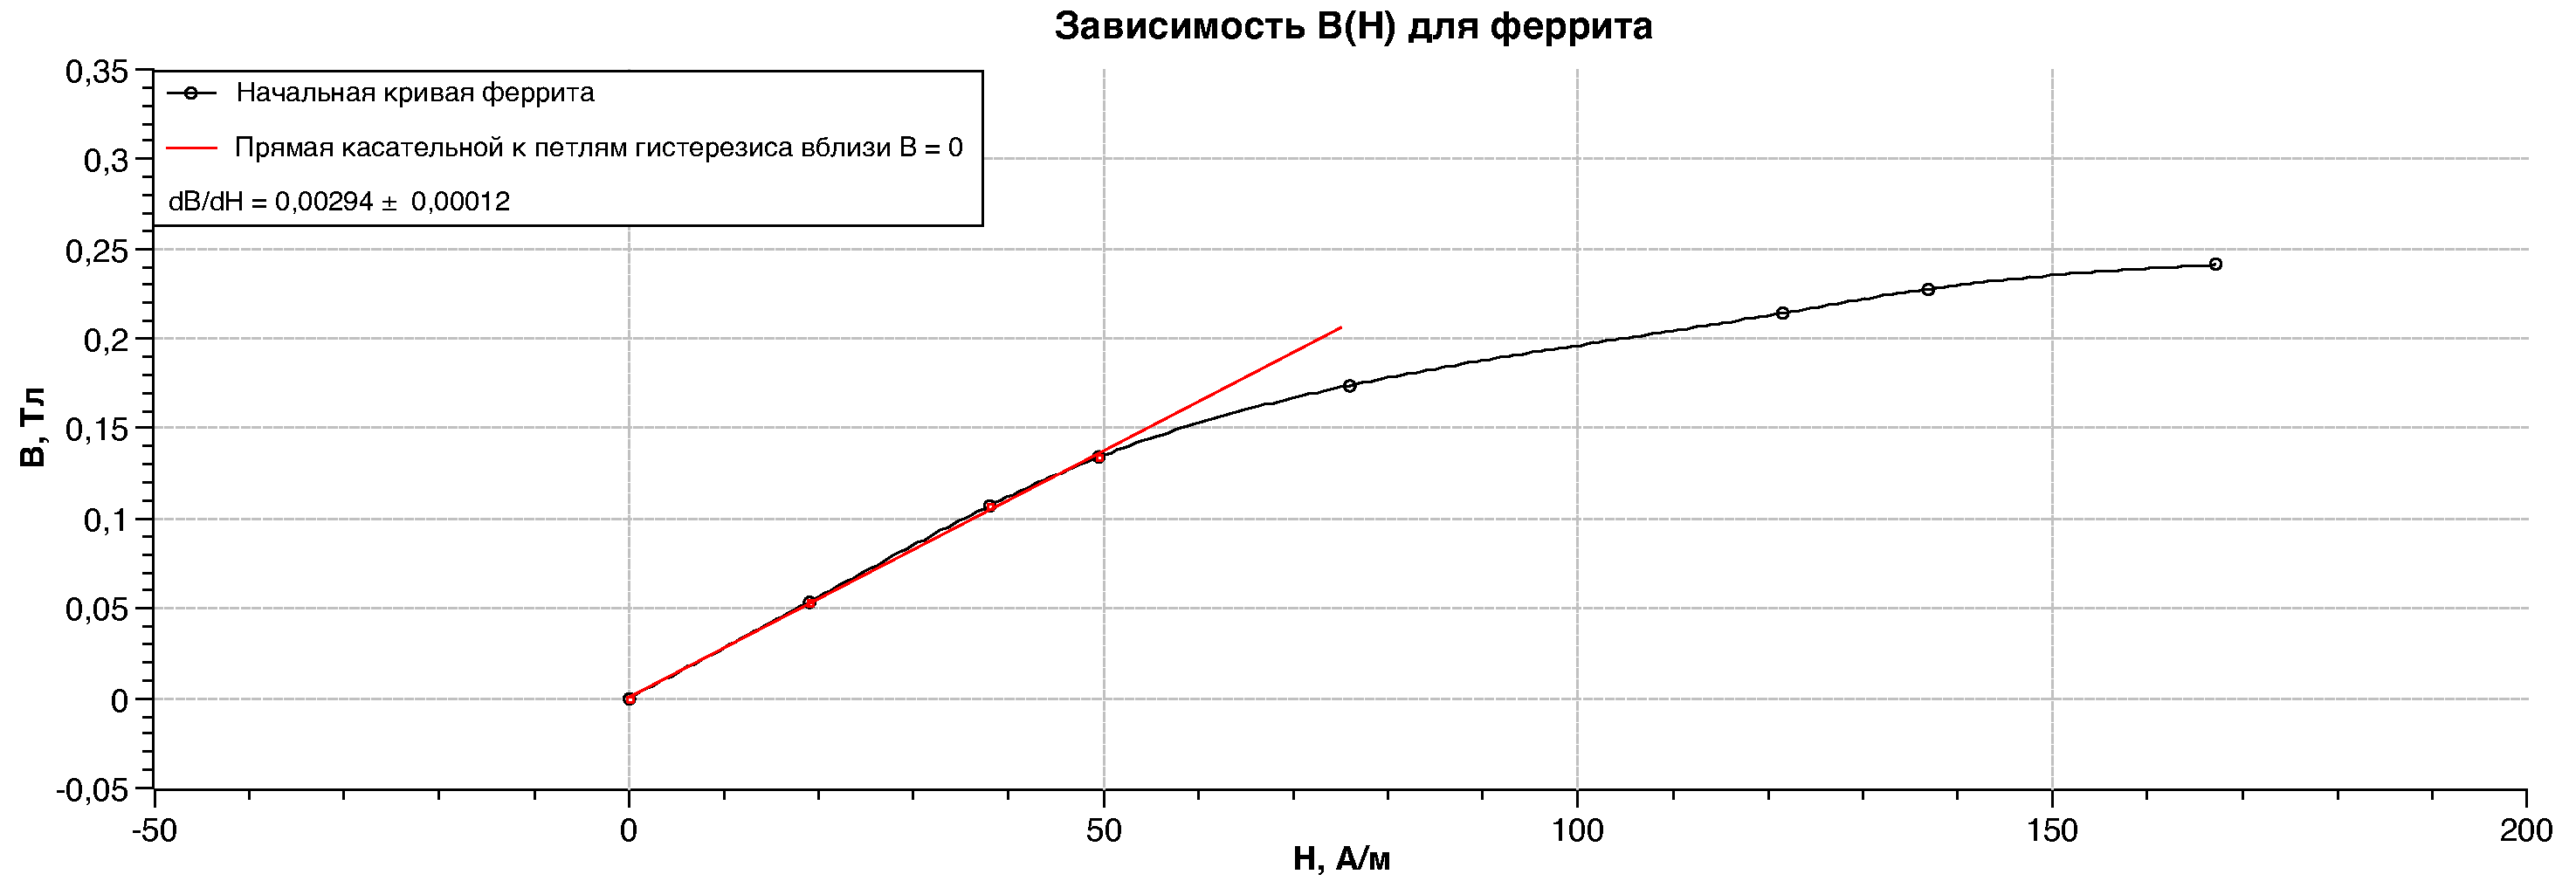
\includegraphics[width = \textwidth]{Image_6}
	\caption{Начальная кривая феррита}
\end{figure}

\newpage

\begin{figure}[h!]
	\centering
	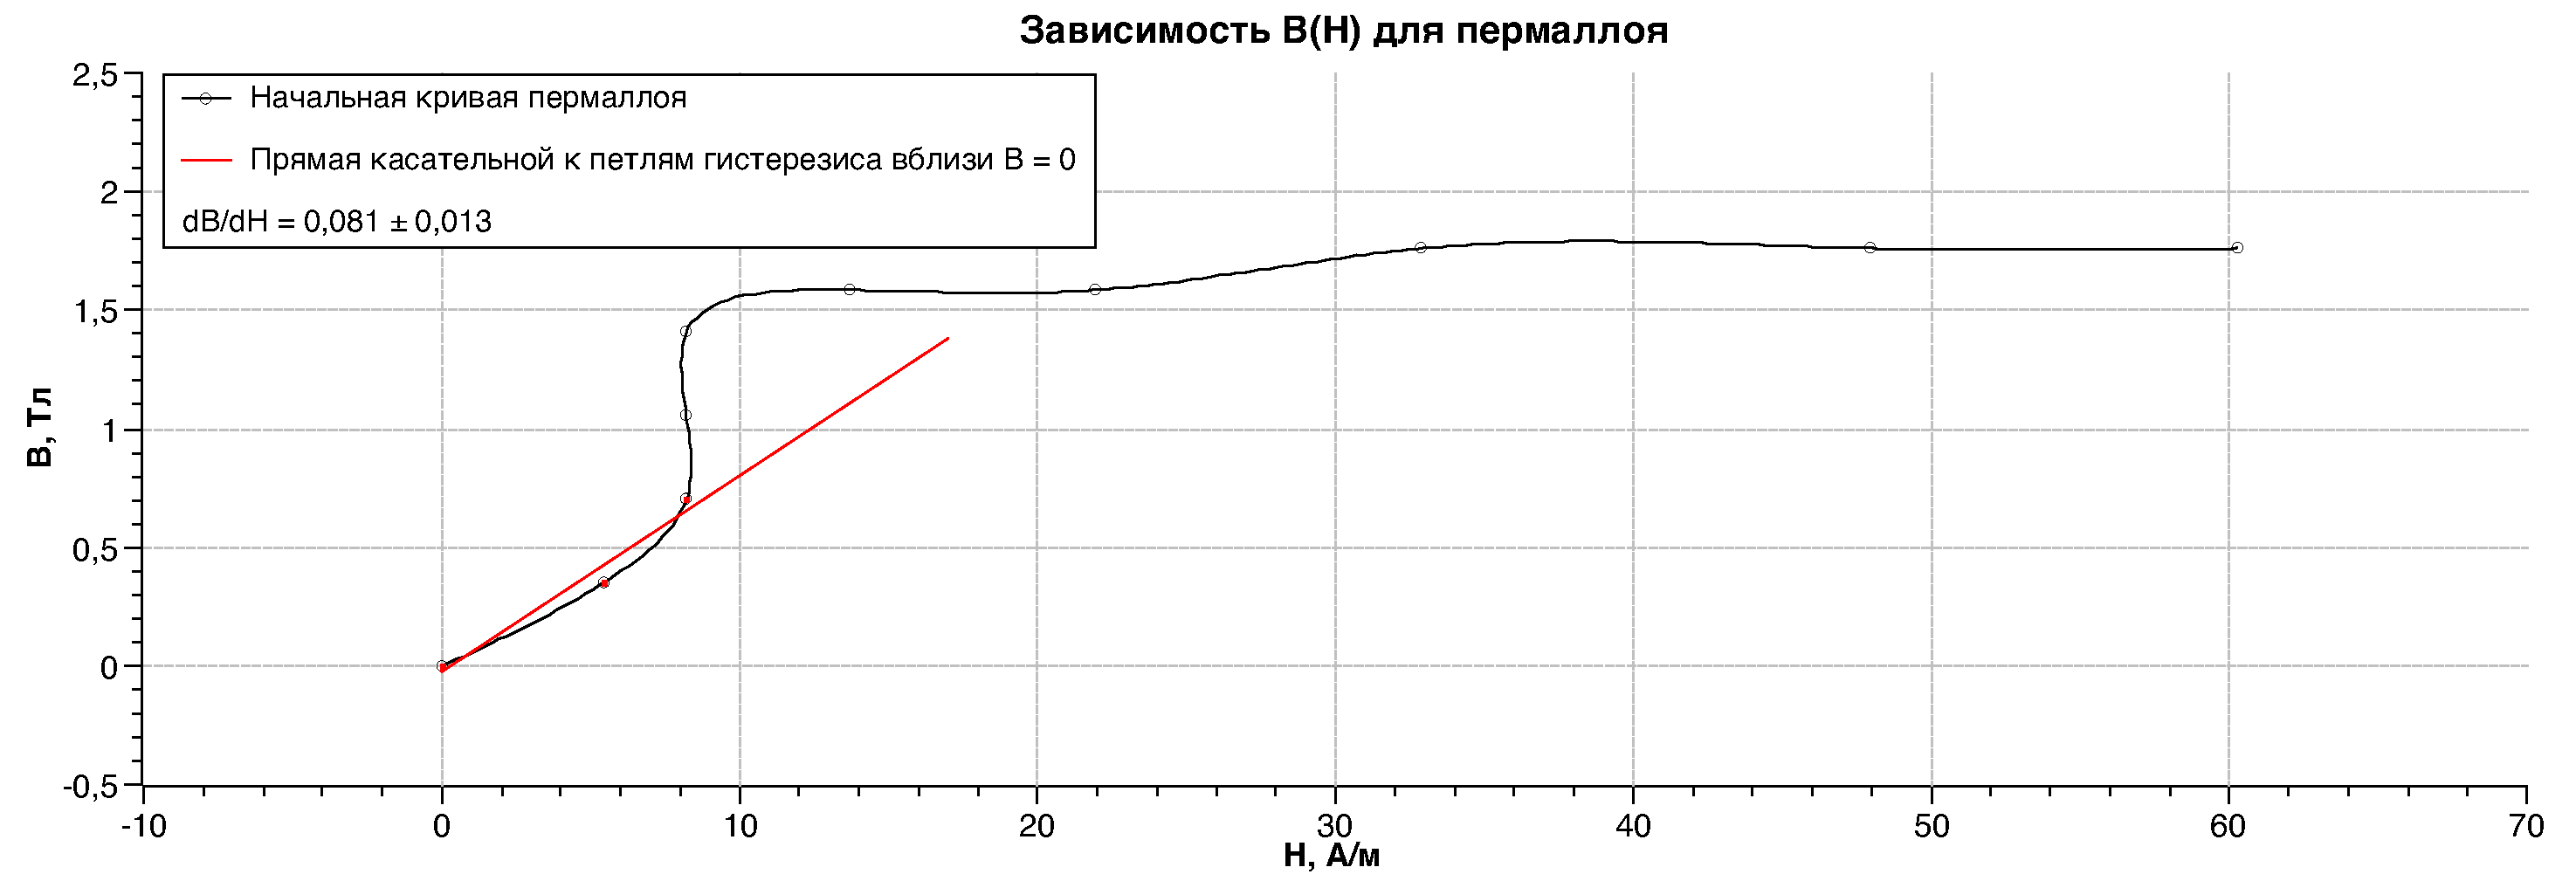
\includegraphics[width = \textwidth]{Image_7}
	\caption{Начальная кривая пермаллоя}
\end{figure}
 \[
 \mu_{max} = \frac{1}{\mu_0} \frac{dB}{dH}
 \]
 
 \begin{itemize}
 	
 	\item	\textbf{Пермаллой}:
 	
 	\fbox{$\mu_{max} \simeq (64,46 \pm 8,30) \times 10^3 $}
 	
     \item	\textbf{Феррит}:
 	
 		\fbox{$\mu_{max} \simeq (2,339 \pm 0,095) \times 10^3$}
 	
 \end{itemize}

\item Сравнение с табличными значениями:

\begin{center}
	\begin{tabular}{|c|c|c|c|}
		\hline
		& Ампл. & Пермаллой & Феррит \\ \hline
		эксп & \multirow{2}{*}{$H_c$, A/м} & $19,2 \pm 0,5$ & $9,0 \pm 0,2$ \\ \cline{1-1} \cline{3-4} 
		табл &  & 5,6  & 4 - 100 \\ \hline
		эксп & \multirow{2}{*}{$B_s$, Тл} & $1,2 \pm 0,06$  & $0,1330 \pm 0,0002$ \\ \cline{1-1} \cline{3-4} 
		табл &  & 1,08 &  0,1-0,4 \\ \hline
		эксп & \multirow{2}{*}{$\mu_{max} \times 10^3$} & $64,46 \pm 8,30$  & $6,0 \pm 0,2$ \\ \cline{1-1} \cline{3-4} 
		табл &  & $10 $ &  0,5 - 20 \\ \hline
	\end{tabular}\\
	\textbf{Таблица 6.} Сверка с табличными значениями.
\end{center}

\end{enumerate}

\end{document}